\documentclass[aspectratio=169,11pt]{beamer}

\usetheme{metropolis}
\metroset{block=fill, numbering=fraction, progressbar=frametitle}

\usepackage[T1]{fontenc}
\usepackage{amsmath,amssymb,bm}
\usepackage{booktabs}
\usepackage{graphicx}
\usepackage{xcolor}

% figures from the simulation-output folders (combined first)
\graphicspath{{../cascaded_chi3/figures/combined/}%
              {../cascaded_chi3/figures/design6/}%
              {../cascaded_chi3/figures/samples/}}

% shorthands
\newcommand{\chitwo}{\chi^{(2)}}
\newcommand{\chithree}{\chi^{(3)}}
\newcommand{\chicasc}{\chi^{(3)}_{\mathrm{casc}}}
\newcommand{\chinat}{\chi^{(3)}_{\mathrm{native}}}
\newcommand{\Dom}{\Delta\omega}
\newcommand{\gtwo}{\gamma_2}
\definecolor{good}{HTML}{2ca02c}
\definecolor{bad}{HTML}{d62728}
\definecolor{d6}{HTML}{9467bd}
\newcommand{\yes}{\textcolor{good}{\textbf{yes}}}
\newcommand{\no}{\textcolor{bad}{\textbf{no}}}

\title{Cascaded $\chitwo{:}\chitwo \to \chithree$ in single-resonance
       LiNbO$_3$ metasurfaces}
\date{\today}

\begin{document}

\maketitle

% ===============================================================
\begin{frame}{The idea, and the metric}
  \textbf{Cascaded Kerr.} Two $\chitwo$ steps synthesise an effective Kerr
  response on the pump; the second harmonic is eliminated adiabatically:
  \[
    \omega_1+\omega_1 \xrightarrow{\ \chitwo\ } 2\omega_1
    \xrightarrow{\ \chitwo\ } \omega_1 ,
    \qquad
    \chicasc(\Dom)= -\,\frac{\omega_1\,|\chitwo|^2\,\eta_{\rm geom}}
                              {6\,n_2^2\,(\Dom+i\gtwo/2)} .
  \]
  \textbf{Single-resonance (SH-only) case:} only the $2\omega_1$ mode is
  resonant --- far easier to fabricate than a two-mode device.

  \begin{alertblock}{The figure of merit}
    \[
      R \equiv \frac{|\chicasc|}{|\chinat|}\;\propto\; Q_2\cdot\eta_{\rm geom}
        \;\propto\; Q_2\cdot(\text{SHG overlap})^2 .
    \]
    $R>1$: the cascade beats the material's own Kerr. Operating point:
    conservative $\Dom=+2\gtwo$.
  \end{alertblock}
\end{frame}

% ===============================================================
\begin{frame}{Five LiNbO$_3$ candidates}
  \small
  \begin{table}
  \centering
  \begin{tabular}{@{}lccccc c@{}}
    \toprule
    & $\lambda_1$ & $Q_2$ & SHG overlap & $\eta_{\rm geom}$ & $R$ & beats native? \\
    \midrule
    S1 & 997\,nm  & 3442 & 0.12 & 0.014 & 0.49 & \no \\
    S2 & 975\,nm  & 3486 & 0.11 & 0.011 & 0.39 & \no \\
    S3 & 1058\,nm & 4641 & 0.19 & 0.037 & 1.76 & \yes \\
    S4 & 1064\,nm & 5633 & 0.21 & 0.044 & \textbf{2.49} & \yes \\
    \textcolor{d6}{\textbf{D6}} & \textbf{1757\,nm} & \textbf{924} & \textbf{0.43} & \textbf{0.18} & \textbf{1.81} & \yes \\
    \bottomrule
  \end{tabular}
  \end{table}
  \begin{itemize}\setlength\itemsep{1pt}
    \item S1--S4: pure-LiNbO$_3$ pillars, height asymmetry, green SH.
    \item \textcolor{d6}{\textbf{D6}}: \textbf{TiO$_2$/LiNbO$_3$ hybrid}, etch-angle asymmetry
          ($0^\circ/90^\circ$), pump at $1.76\,\mu$m.
  \end{itemize}
  % \footnotesize
  % \alert{Normalisation caveat:} S1--4 use an \emph{area}-normalised overlap, D6 a
  % \emph{volume}-normalised one; the absolute cross-comparison of $R$ rests on the shared
  % $O(1)$ calibration factor $C_{\rm bridge}=1$. Ranking within each is robust.
\end{frame}

% ===============================================================
\begin{frame}{Enhancement over the native Kerr}
  \centering
  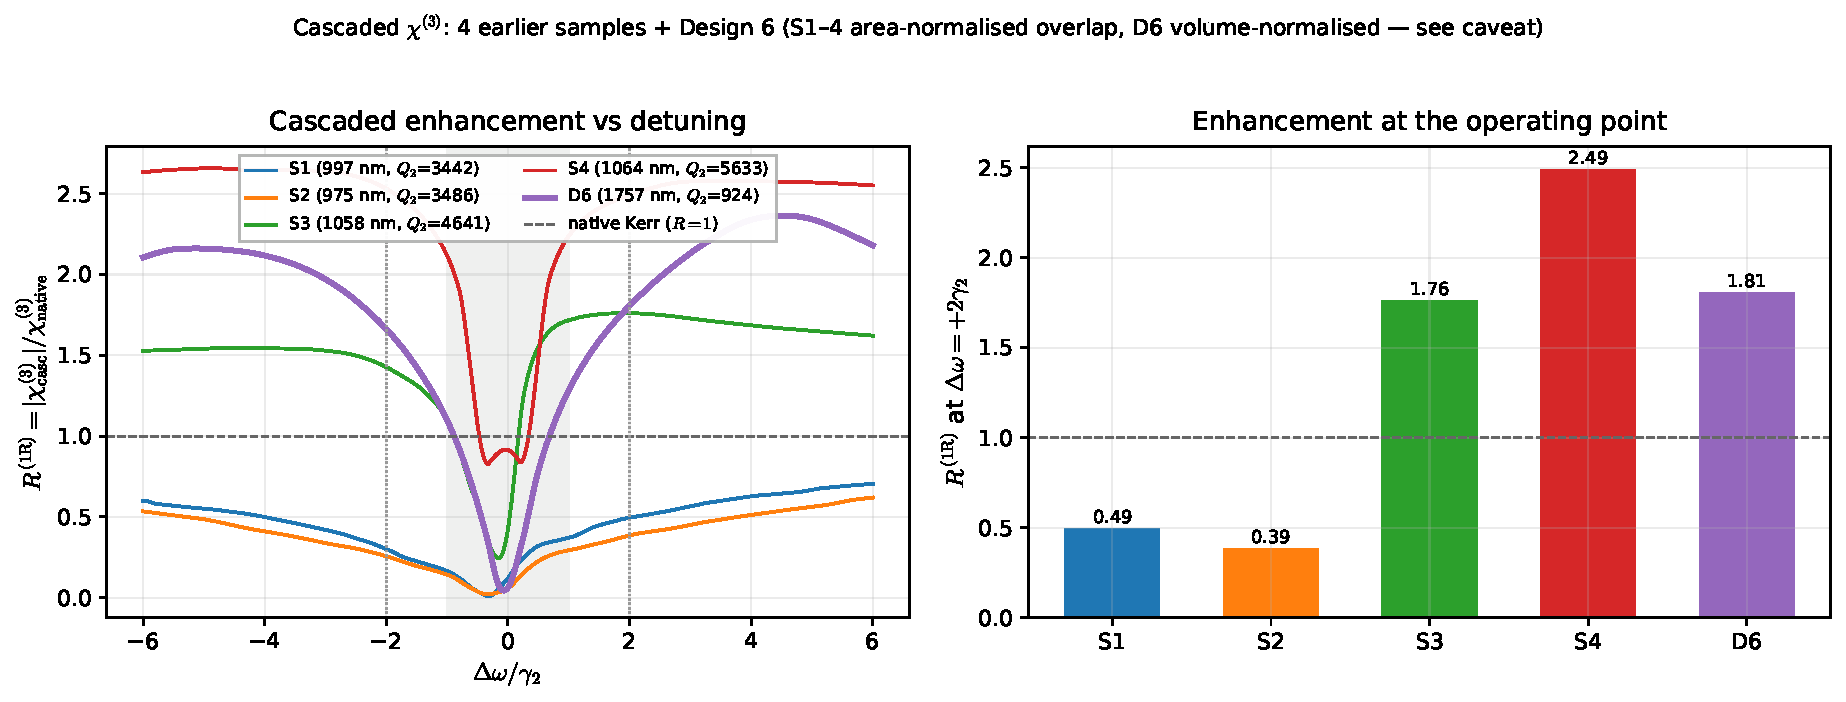
\includegraphics[width=0.98\linewidth]{combined_R_comparison}
  \\[2pt]
  \footnotesize Only \textbf{S3, S4, D6} exceed $R=1$. Ideal-limit winner: \textbf{S4}
  ($R=2.49$). The overlap is small at resonance (Fano dip), so the wings are used.
\end{frame}

% ===============================================================
\begin{frame}{Two routes to the same $R$}
  \begin{columns}[T]
    \begin{column}{0.6\linewidth}
      \centering
      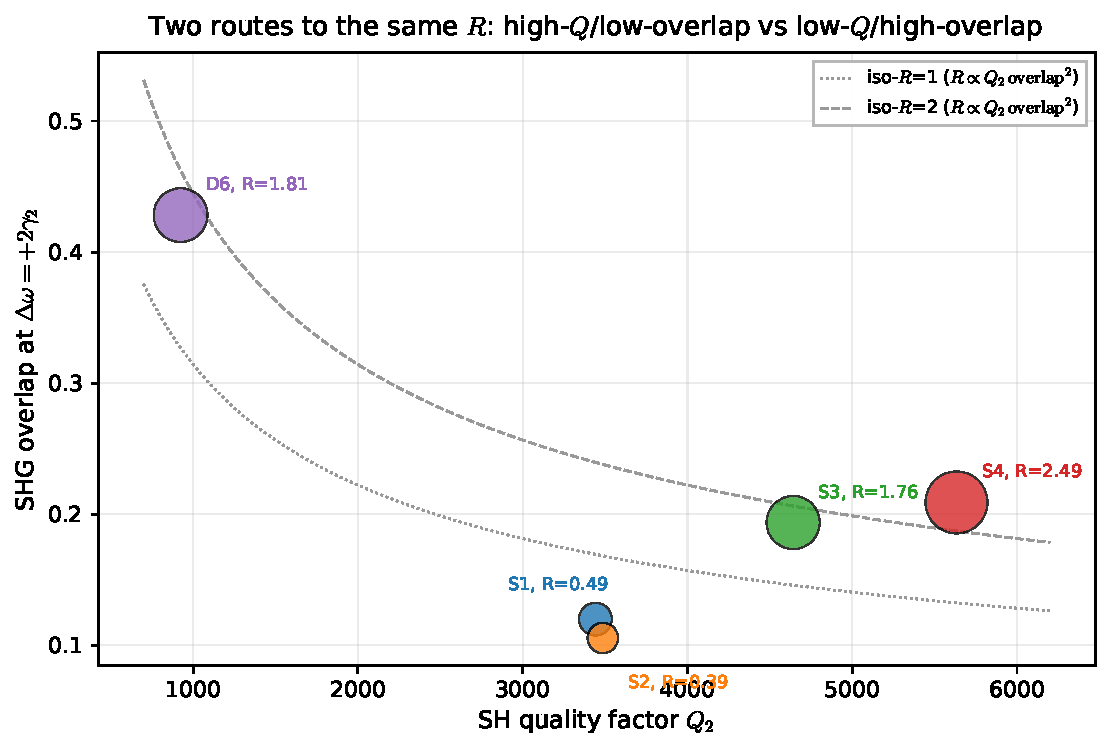
\includegraphics[width=\linewidth]{combined_tradeoff}
    \end{column}
    \begin{column}{0.4\linewidth}
      \small
      Since $R\propto Q_2\,(\text{overlap})^2$:
      \begin{itemize}\setlength\itemsep{4pt}
        \item \textbf{S3/S4:} high $Q_2$ ($\sim$5000), modest overlap ($\sim$0.2).
        \item \textcolor{d6}{\textbf{D6:}} low $Q_2$ (924), \textbf{high overlap} (0.43).
      \end{itemize}
      \vspace{4pt}
      Both reach $R\approx2$ --- but they behave very differently in a
      \emph{real, pulsed} experiment.
    \end{column}
  \end{columns}
\end{frame}

% ===============================================================
\begin{frame}{The catch: a real ps pulse is spectrally broad}
  \centering
  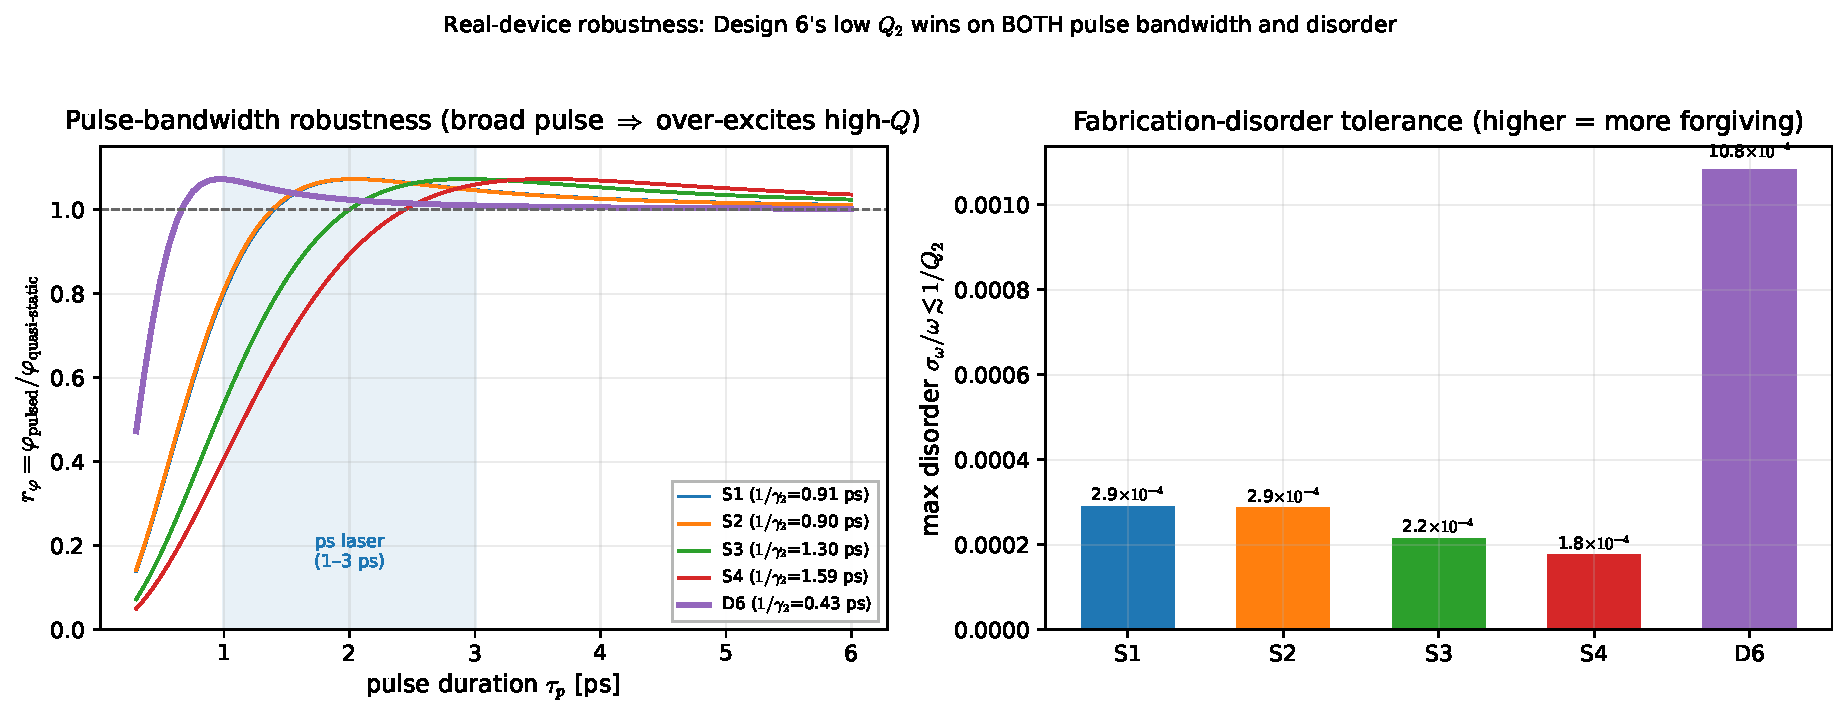
\includegraphics[width=0.98\linewidth]{combined_real_device}
  \\[2pt]
  \footnotesize
  A $\tau_p{=}1$--$3$\,ps pulse has bandwidth $\sim$\,$0.5\,\text{THz}/\tau_p[\text{ps}]$.
  For \textbf{high-$Q$} designs this \emph{exceeds} the linewidth: up to \textbf{22\%} of the
  generated SH lands at the \emph{wrong} detuning sign (cancellation) $\Rightarrow$ the Kerr
  phase collapses ($r_\varphi{=}0.4$ at 1\,ps for S4). \textcolor{d6}{\textbf{D6}}'s broad linewidth
  keeps the pulse clean ($r_\varphi\!\approx\!1$) \emph{and} tolerates $5\times$ more fabrication disorder.
\end{frame}

% ===============================================================
\begin{frame}{Which is best?}
  \begin{columns}[T]
    \begin{column}{0.5\linewidth}
      \begin{block}{Ideal limit}
        \textbf{S4}, $R=2.49$. \\[3pt]
        Highest $Q_2$, best raw enhancement --- \emph{if} the design $Q$ is reached and
        the pulse is long enough ($\tau_p\gtrsim3$\,ps).
      \end{block}
    \end{column}
    \begin{column}{0.5\linewidth}
      \begin{alertblock}{Real fabricated device}
        \textcolor{d6}{\textbf{D6}}, $R\approx1.8$. \\[3pt]
        Nearly the same enhancement, but \textbf{robust}: no pulse-bandwidth penalty at
        1--3\,ps, $5\times$ looser disorder tolerance, low $Q$ reliably fabricated.
      \end{alertblock}
    \end{column}
  \end{columns}
  \vspace{4pt}
  \centering
  \small High-$Q$ wins on paper; \textbf{low-$Q$/high-overlap wins in the lab, at least
  theoretically}.
\end{frame}

% ===============================================================
\begin{frame}{What we measure in the experiment (my subjective -- open to discussion)}
  \textbf{Closed-aperture Z-scan vs.\ pump detuning} --- the cascade's fingerprint.
  \begin{itemize}\setlength\itemsep{3pt}
    \item Pump always at $\omega_1$; scan the pump wavelength ($\sim$1\,nm) so the generated
          $2\omega_1$ sweeps across the SH resonance, $\Dom:-\!\to\!+$.
    \item \textbf{Sign flip:} valley$\to$peak (self-focusing) $\to$ peak$\to$valley
          (defocusing) as $\Dom$ crosses zero. The cascade is \emph{odd} in $\Dom$;
          native Kerr is a constant background $\Rightarrow$ isolate the cascade as the
          antisymmetric part.
    \item \textbf{SHG conversion efficiency} in the same sample calibrates the absolute
          $\chithree$ scale (pins $C_{\rm bridge}$).
  \end{itemize}
  \begin{block}{Regime}
    ps pulses, $\tau_p\!\sim\!1$--$3$\,ps at $\lambda_1\!\approx\!1.76\,\mu$m (available).
    D6's SH lifetime $1/\gtwo\!\approx\!0.43$\,ps $\Rightarrow$ quasi-static, sign flip
    stays sharp.
  \end{block}
\end{frame}

% ===============================================================
\begin{frame}{Is it achievable in a real device? Preliminary analysis}
  \footnotesize
  \begin{table}
  \centering
  \begin{tabular}{@{}l c p{6.4cm}@{}}
    \toprule
    Goal & Verdict & Why \\
    \midrule
    Beat native Kerr, $R>1$ & \yes & $R\approx1.8$--$2.5$ (S3/S4/D6); robust to the $O(1)$ scale uncertainty \\
    \emph{Measure} the cascade (sign flip) & \yes & antisymmetric-in-$\Dom$ signature; cleanest on \textcolor{d6}{\textbf{D6}} \\
    CW Kerr \emph{device} & \no & single-pass phase is $\mu$rad even at damage --- need a two-mode cavity \\
    Reach the \emph{designed} high $Q$ & \alert{risk} & disorder caps S4 first ($\sigma_\omega/\omega\!\lesssim\!2\times10^{-4}$) \\
    \bottomrule
  \end{tabular}
  \end{table}
  \vspace{2pt}
  \textbf{Honest uncertainties.} Absolute $R$ is order-of-magnitude ($C_{\rm bridge}$, native
  $\chithree$ at these wavelengths, the area/volume overlap convention). The \emph{sign},
  \emph{ranking}, and $Q/\eta$ scaling are far more robust than the absolute number.
\end{frame}

% ===============================================================
\begin{frame}{Bottom line}
  \begin{alertblock}{Recommendation}
    Run the ps-pulsed \textbf{Z-scan sign-flip} measurement on \textcolor{d6}{\textbf{Design 6}}
    at $\lambda_1\!\approx\!1.76\,\mu$m, with an SHG-efficiency calibration in the same sample.
  \end{alertblock}
  \begin{itemize}\setlength\itemsep{2pt}
    \item \textbf{S4} has the highest ideal $R$ (2.49) but is the most fragile
          (needs $\tau_p\!\gtrsim\!3$\,ps and sub-$2\times10^{-4}$ disorder).
    \item \textcolor{d6}{\textbf{D6}} gives $R\approx1.8$ (up to $\sim$2.4 in the wings) and is
          robust on \emph{both} pulse bandwidth and fabrication disorder --- the best
          design to actually \emph{see} the cascaded $\chithree$.
    \item The achievable observable is the \textbf{sign flip}.
  \end{itemize}
  \vspace{2pt}
  % \centering\footnotesize
  % Next: pin $C_{\rm bridge}$ with one absolute SHG number; refine $\chinat$ at 1.76\,$\mu$m.
\end{frame}

\end{document}
